\documentclass[10pt, a4paper]{arbeitsblatt}

\ladeModule{theme,boxen}
\ladeFach[]{informatik}

\aboptionen{
	name		= {J. Neugebauer},
	kuerzel		= {Ngb},
	titel		= {Die Schlange (Queue)},
	reihe		= {Lineare dynamische Datenstrukturen},
	fach		= {Informatik},
	lerngruppe	= {Q1},
	nummer		= {II.01},
	lizenz		= {cc-by-nc-sa-4},
	version		= {2021-11-23},
}

\begin{document}
\ReiheTitel


\begin{rahmen}
	\subsection*{Beim Arzt}

	In der Sprechstunde beim Arzt werden Patient:innen in der Reihenfolge behandelt, in
	der sie ankommen. Zuerst kommt Sara, dann Paul und schließlich Maren. Dann wird
	eine Patient:in ins Behandlungszimmer gerufen. Während die erste Patient:in in
	Behandlung ist, trifft Ida ein.
\end{rahmen}

\begin{aufgabe}[icon=\Large\iconPartner]
Stellt die Veränderungen der Patient:innenwarteschlange
grafisch dar.
\end{aufgabe}

\begin{aufgabe}[icon=\Large\iconPartner]
Vergleicht eure Darstellung mit dem Bild unten und
erklärt die Bedeutung
der Befehle \code{enqueue} und \code{dequeue}.

\begin{center}
	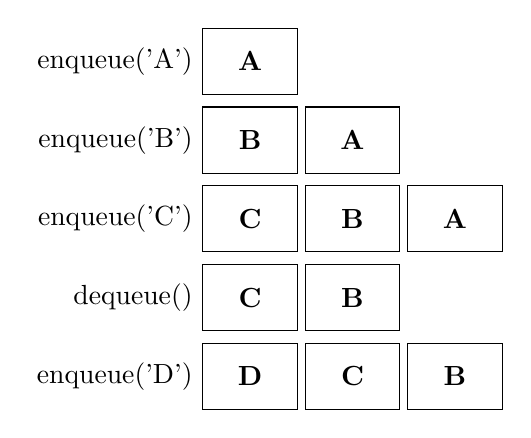
\begin{tikzpicture}[box/.style={draw,rectangle,inner sep=.3cm,node distance=1cm,minimum width=1.2cm,font={\bfseries}}]
		\node[box,label=left:{\code{enqueue('A')}}] (A1)
		{A};
		\node[box,below of=A1,label=left:{\code{enqueue('B')}}] (B1)
		{B};
		\node[box,right of=B1,xshift=.3cm] (A2) {A};
		\node[box,below of=B1,label=left:{\code{enqueue('C')}}] (C1)
		{C};
		\node[box,right of=C1,xshift=.3cm] (B2) {B};
		\node[box,right of=B2,xshift=.3cm] (A3) {A};
		\node[box,below of=C1,label=left:{\code{dequeue()}}] (B3)
		{C};
		\node[box,right of=B3,xshift=.3cm] (A4) {B};
		\node[box,below of=B3,label=left:{\code{enqueue('D')}}] (D1)
		{D};
		\node[box,right of=D1,xshift=.3cm] (B4) {C};
		\node[box,right of=B4,xshift=.3cm] (A5) {B};
	\end{tikzpicture}
\end{center}
\end{aufgabe}

\begin{aufgabe}[icon=\Large\iconPartner]
Die hier vorgestellte Datenstruktur wird in der
Informatik als \emph{Schlange} (englisch \emph{Queue}) bezeichnet. Eine Schlange arbeitet nach
dem Verarbeitungsprinzip \enquote{First In - First Out} (\emph{FIFO}).

\begin{teilaufgaben}
	\teilaufgabe
	Erklärt die Herkunft der Bezeichnung \enquote{First In - First Out} anhand der
	Darstellungen aus Aufgabe 1 bis 3.
	\teilaufgabe
	Beschreibt das \emph{FIFO}-Prinzip mit eigenen Worten.
\end{teilaufgaben}

\begin{center}
	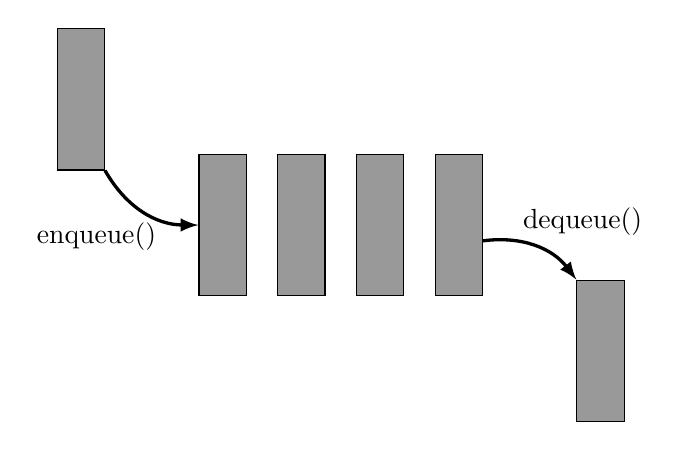
\begin{tikzpicture}[box/.style={draw,rectangle,fill=black!40,minimum width=.6cm,minimum height=1.8cm}]
		\node[box] (b1) {};
		\node[box,right of=b1] (b2) {};
		\node[box,right of=b2] (b3) {};
		\node[box,right of=b3] (b4) {};
		\node[box,left of=b1,xshift=-.8cm,yshift=1.6cm] (b5) {};
		\node[box,right of=b4,xshift=.8cm,yshift=-1.6cm] (b6) {};

		\path[->,>=latex,auto,very thick] (b5.south east) edge[bend right]
		node [below,xshift=-.6cm] {\code{enqueue()}} (b1.west)+(0,.2);
		\path[->,>=latex,auto,very thick] (b4.east)+(0,-.2) edge[bend left]
		node [above,xshift=.6cm] {\code{dequeue()}} (b6.north west);
	\end{tikzpicture}
\end{center}
\end{aufgabe}

\end{document}
